\documentclass[11pt,a4paper]{article}

\usepackage{jheppub}
\usepackage{dsfont}
\usepackage{nicefrac}
\usepackage{bm}
\usepackage{mathsettings}
\usepackage{xparse}
\usepackage{mathrsfs}
\usepackage[none]{hyphenat}
\usepackage{tabularx}
\usepackage{makecell}
\usepackage{empheq}
\usepackage{pifont}

\newcommand{\bfnt}[1]{{\bfseries #1}}
\newcommand{\ifnt}[1]{{\itshape #1}}

% https://tex.stackexchange.com/a/531829/200495
\makeatletter
\gdef\@fpheader{}
\makeatother


\begin{document}

	\title{A Brief Primer on X-ray Diffraction Crystallography}
	\author{Wrichik Basu}
	\affiliation{Dept. of Physics, Scottish Church College, University of Calcutta}
	\date{\today}
	
	\maketitle
	
	\section{Introduction}
	
	\section{Spectroscopy vs. Crystallography}
	
		\textbf{Spectroscopy} is the study of absorption and/or emission of electromagnetic radiation in which the incident radiation interacts with the molecule and produces characteristic signals. From spectroscopy, we can get the following data about a molecule: %
%			
			\begin{itemize}%
%		
			    \item Bond lengths and bond angles of simple (diatomic, triatomic) molecules.
			    
			    \item Combination of Infrared and NMR (${}^1 \mathrm{H}$ and ${}^{13} \mathrm{C}$) spectroscopy provides information about functional groups, bond connectivity and stereochemistry (absolute configuration) of simple molecules.
		    
		    \end{itemize}
		    
		Spectroscopy, however, cannot provide information about bond lengths, bond angles, torsion angles, etc. of complicated molecules.
		
		\textbf{Crystallography}, on the other hand, deals in the interaction of EM radiation of very small wavelength ($\lambda \sim \SI{1}{\angstrom}$) with solid materials (crystalline or amorphous) through scattering. The main difference with spectroscopy is that in crystallography, there is no absorption ot emission of radiation; only scattering of radiation. Crystallography allows us to study%
%			
			\begin{itemize}%
%			
			    \item Accurate bond length, bond angles, torsion angles, precise absolute configuration, etc. of all types of crystalline substances.
			    
			    \item 3D structure of crystalline substances can lead to intermolecular or interionic interactions. Structure property relationship can be obtained using data from crystallography.
			    
			\end{itemize}
			
	\section{Why X-rays?}
	
		
	
	\section{Sources of X-rays}
	
		For X-ray diffraction experiments, monochromatic radiation from various metal-based sources (eg. Cu, Ag, Mo) is used in the lab. There are also synchotron-based sources for X-rays.%
%			
			\begin{itemize}%
%			
			    \item \bfnt{Sealed-tube X-ray sources}%
%			    	
			    	\begin{itemize}[label={$\hookrightarrow$}]%
%			    	
			    	    \item \ul{Fine focus sources}: Operate at around $50~\si{kV}$ and $40~\si{mA}$ ($\sim \SI{2}{kW}$). Can give a photon flux of around $\SI{1e7}{photons/s~mm^2}.$
			    	    
			    	    \item \ul{Microfocus sources}: Highly focussed beam. Operates at $40-50~\si{kV}$ and $2-15~\si{mA}$  ($<\SI{1}{kW}$). Can provide around $\SI{1e8}{photons/s~mm^2}.$
			    	    
			    	\end{itemize}
			    	
			    \item \bfnt{Rotating anode based source}: The anode is rotated at a very high speed of around $10,000~\si{rpm}.$ Cu, Mo or dual anode is used. Generally microfocus-based system. Operates at $\SI{60}{kV}$ and $\SI{100}{mA}$ or higher ($> \SI{6}{kW}$). Can produce a flux $\sim \num{1e10}-\num{e11}~\si{photons/s~mm^2}.$
			    
			    \item \bfnt{Metal Jet source}: Liquid Gallium is used, giving $\lambda = \SI{1.340}{\angstrom}.$ High intensity at much low power. Can generate $\sim \num{1e11}-\num{e12}~\si{photons/s~mm^2}.$
			    
			    \item Synchotron Sources:
			    
			\end{itemize}
	
	\section{Generating X-rays}
	
		Fig.~XXXX shows the schematic of a X-ray tube. The potential difference between the anode to cathode is around $20-60~\si{kV},$ while the Tungsten filament is supplied a current of $\sim 2-50~\si{mA}.$ The target is composed of the material from which we want to generate the X-rays (generally Cu, Mo or Ag). The Be-window provides a transparent window for the generated X-rays to pass through.
		
		The tube is not allowed to cool down between experiments. In the stand-by state, the filament current is reduced to around $\SI{5}{mA}$ and the anode potential is also reduced to $\SI{20}{kV}.$ When data collection is started, the anode voltage is increased to $>\SI{50}{kV}$ and the current in the Tungsten filament is increased to $\SI{40}{mA}.$ In this state, the heated Tungsten filament generates electrons, which are then accelerated and finally hit the target at the anode.
		
		These electrons are able to knock out electrons from the K-shell of an atom in the target. Once an electron is removed from the K-shell, electrons from higher energy levels release energy and come to the K-shell. This release energy is the characteristic X-rays of the material. There are three possible transitions which give rise to X-rays of three different wavelengths. These are shown in Fig.~XXXX.
		
		The X-ray spectra of Cu and Mo are shown in Fig.~XXX. The $K_\alpha$ peaks are very close to each other, and are shown magnified in Fig.~XX. The background radiation is attributed to Bremstrahlung, which is the radiation emitted by electrons when they are decelerated in the X-ray tube. The corresponding wavelengths can be found in table~XX.
		
		We want to use monochromatic radiation for X-ray diffraction experiments. For this, we have to filter out the unwanted $K_\beta$ and $K_{\alpha2}$ radiations. To filter the $K_\beta$ spectra, we use a $\beta$-filter. The  $\beta$-filters used for Cu and Mo are listed in table~XX. To separate $K_{\alpha1}$ from $K_{\alpha2}$, we use a crystal monochromator.
	
	\section{The physics behind X-ray diffraction}
	
	
	\section{Type of X-ray diffraction experiments}
	
	
	
	\section{Mounting a crystal on SCXRD diffractometer}
	
		\begin{figure*}[t]
			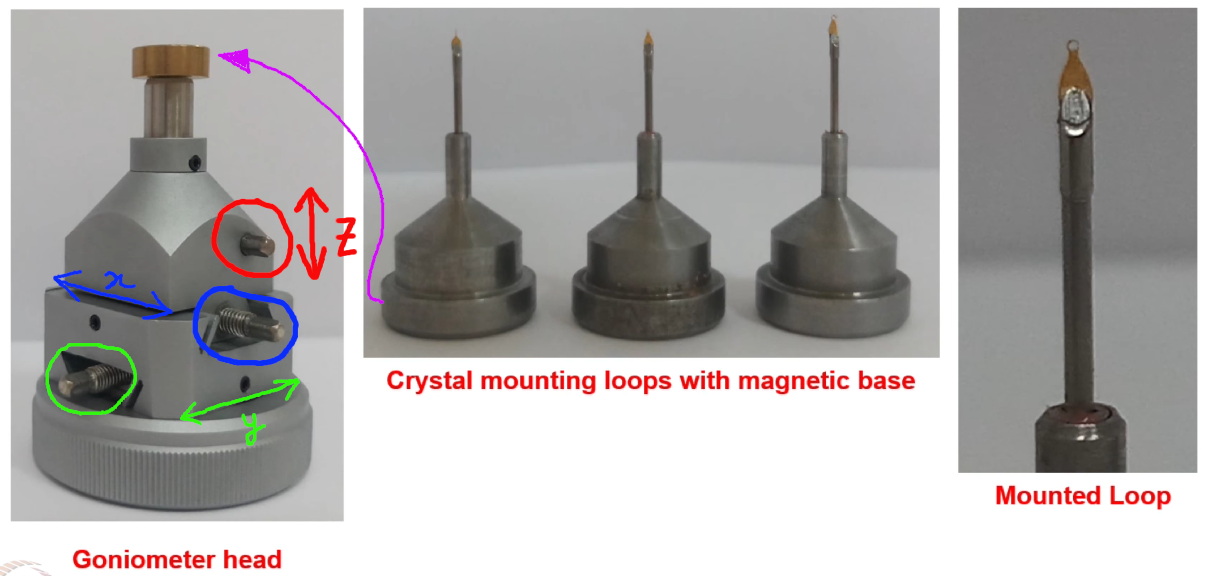
\includegraphics[scale=0.5]{goniometer_mod.png}
			\caption{\label{fig:goniometer}The goniometer head, mounting loop with the mounting base.}
		\end{figure*}
	
		In fig.~\ref{fig:goniometer}, a goniometer head is shown. This head is mounted on the goniometer of the diffractometer. The top of the goniometer head is a magnetic base which allows the mounting loops to be held in place. To align the crystal in the X-ray beam, the goniometer head has three screws that allow movement in the three Cartesian directions. These screws and their respective directions have been demarcated in the figure.

		The tip of the mounting metal pin has a small polymer loop. The crystal is mounted on this loop using some thick oil, which keeps the crystal in place by its surface tension. These loops are available in various diameters, generally in the range $0.05-0.5~\si{mm}.$

		Nylon loops are also available, in which the loop is made by a nylon thread, which is then twisted several times and then glued to a pin. The pin is attached to a brush, which can be directly mounted on the goniometer head and placed in the X-ray beam.
		
	\section{Selection of crystals for SCXRD}
	
		
	
		We cannot know whether a crystal is good or bad until we mount it on the diffractometer and put it in the path of X-rays. Therefore, when a crystal passes the above minimum selection criteria, we mount it on the goniometer head and shine X-rays on it. The axis about which the crystal is mounted is known as the $\phi$ axis. We rotate crystal about the $\phi$ axis through a full $2\pi$ rotation while keeping the X-ray on for 1-2 minutes depending on the size of the crystal, and we keep recording the diffraction pattern. The diffraction pattern thus recorded is known as the \bfnt{rotation photograph} of the single crystal.
		
		\begin{figure*}[h]
			\centering
			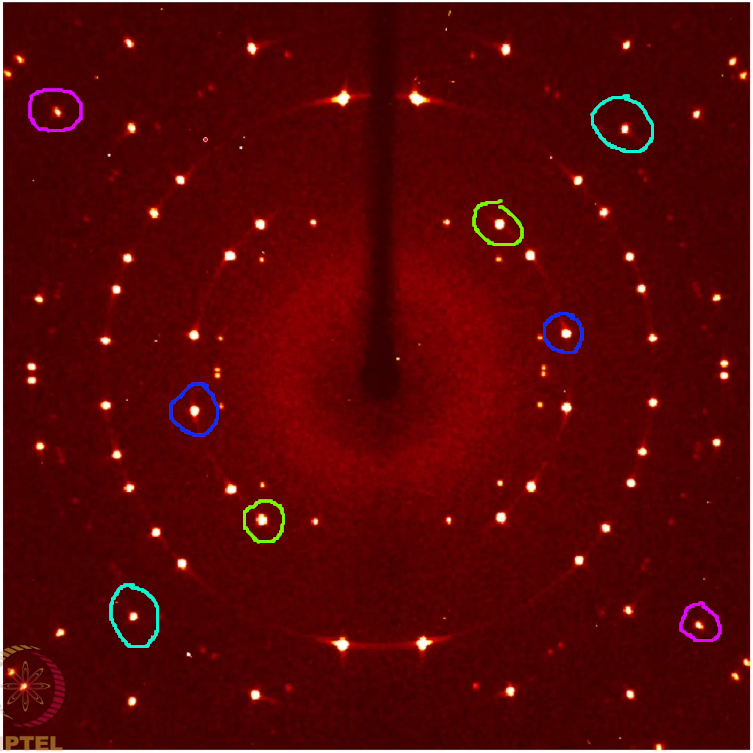
\includegraphics[scale=0.3]{rotation_photograph_mod.png}
			\caption{\label{fig:rotation_photo}Rotation photograph of a single crystal. Each spot has another spot on the other side related by a centre of inversion. Some examples are shown by different coloured circles; two spots encircled by the same colour are related to each other. The dark shadow is that of the beam stop, which prevents the direct X-ray beam from falling on the detector.}
		\end{figure*}
		
		Figure~\ref{fig:rotation_photo} shows the rotation photograph of a single crystal. This photograph is always centro-symmetric irrespective of the type of crystal geometry. Each spot on the rotation photograph has another corresponding spot that is related to it by a centre of inversion. If instead of these spots, the rotation photograph is composed of concentric circles, we conclude that the crystal is not a single crystal, but a polycrystal, and is not suitable for XRD.

	
	\section{The SCXRD diffractometer and its types}
	
	\section{How much data do we have to collect?}
	
	
		

\end{document}